\documentclass{article}
\usepackage{syntax}
\usepackage{tikz}
\usepackage{fancyvrb}
\usetikzlibrary{automata, positioning}

\begin{document}
    %Fachlexikon für definition verwenden
    \newpage
    \tableofcontents
    %Einleitung
    \newpage
    \section{Einleitung}
    \subsection{Aufgabe und Motivation}
    \subsection{Aufbau der Arbeit}
    Die vorliegenede Arbeit setzt sich aus TODO nachfolgenden Kapiteln zusammen. 
    Im zweiten Kapitel TODO
    Anschließend daran wird im dritten Kapitel TODO
    Darauf aufbauen wird im vierten und fünften Kapitel TODO
    Der Fokus im letzten Kapitel liegt auf TODO 
    \newpage
    \section{Terminologie}
    Der Fokus dieses Kapitels liegt auf der Definition zentraler Fachbegriffe und dadurch einen einheitlichen terminologischen Rahmen zu schaffen. Das Ziel dieses Kapitels ist es die Verständlichkeit der nachfolgenden Kapitel zu erhöhen und die theoretischen Grundlagen der Arbeit zu festigen.\\
    \textbf{Schleifen} \par
    Eine Schleife ist eine Kontrollstruktur, die einen Programm-Abschnitt mehrmals ausführt. \cite{22}
    Häufig ist dabei die Schleife die zeitintensivste Komponente eines Programms, da ihre die Ausführung sehr viel Zeit in anspruch nehmen kann. \cite{1}
    Der Algrorithmus dieser Kontrollstruktur kann dabei iterativ oder rekursiv implementiert werden. Beide Ansätze haben dabei das gleiche Ziel, aber setzen die Schleife anders um. Bei der Iteration wird die Schleife mehrmals wiederholt wird. Bei der Rekursion ruft sich die zu wiederholende Funktions mehrmals selbst auf. \cite{3}
    Die Iteration verwendet dabei einen Akkumulativenansatz. Dabei wird das Problem schrittweise gelöst. Der Prozess wird solange wiederholt bis eine vordefinierte (Abbruch-)Bedingung erfüllt ist. \cite{3}
    Im gegensatz zur Iteration verwendet die Rekursion keinen Akkumulativenansatz, sondern zerlegt das Problam in mehrere (Teil-)Probleme. Für die Teilprobleme werden dann einzelne Lösungen erarbeitet, welche dann kombiniert werden um das eigentliche Problem zu lösen. \cite{3}
    Laut Chen L. spiegelt die Iteration das menschliche Denken wieder, weshalb sie sich besonders für lineare Probleme eignet. 
    Die Rekursion hingegen ist für Probleme geeignet, welche Zwischenergebnisse oder Teillösungen benötigen. \cite{3}
    Eine Schleife kann dabei in zeitabhängig oder horizontal unterteilt werden. Bei einer zeitabhängigen Iteration ist das Ergebniss des aktuellen Schleifendurchlaufs vom Ergebnis des vorherigen Durchlaufs ab. Hingegen bei horizontalen Schleifen die Ergbenisse der einzelnen Schleifendurchläufe unabhängig voneinander sind. \cite{5} \\
    \textbf{Domain Specific Language} \par
    Bei einer domänenspezifische Sprache (DSL) handelt es sich um eine Programmiersprache, die mit dem Ziel entwickelt wurden ist, spezifische Aufgabenstellungen innerhalb eines begrenzten Anwendungskontexts (Domaine) besonders effektiv zu bearbeiten. \cite{18}
    DSLs bilden das Gegenstück zu General-Purpose Languages wie Java, C++ oder Python. \cite{14}
    Dabei verfügen DSLs oftmals über eine reduzierte Syntax, die ausschließlich für den jeweilige Domaine relevant ist. Teilweise wird diese durch eine GPL ergänzt. \cite{18}
    Es wird zwischen externen und internen DSLs unterschieden. Externe DSLs haben ihre eigene Syntax. Dadurch kann eine größere flexibilität geschaffen werden, aber zeitglich ist der Aufwand für den Entwickler sehr hoch, weil alle relevanten Tools selbst implementieren muss. Außerdem braucht der Benutzer länger Zeit um die Syntax zu lernen. \cite{7}
    Zur Laufzeit wird die externe DSLs dann in eine GPL übersetzt. \cite{14}
    Interne DSLs verwenden die Syntax einer GPL und kann über eine Programmierschnittstelle oder Bibliothek aufgerufen werden. \cite{14}
    Die Vorteile von DLSs liegen in ihrer strukturellen Klarheit und Spezialisierung. Dem gegenüber stehen die Nachteile eines hohen Initialaufwands sowie einer begrenzten Flexibilität und Verfügbarkeit. \cite{18} \\ 
    \textbf{Visual Programming Language} \par
    Das Hauptziel visueller Programmiersprachen (VPLs) besteht in der Verbesserung der Darstellung der Programmierlogik sowie in der Erleichterung des Verständnisses von Programmabläufen. \cite{13}
    Dadurch soll der Fokus des Programmierens stärker auf konzeptuelle statt symtaktische Aspekte verlagern. Die syntaktischen Aspekte werden dabei von der Entwicklungsumgebung übernommen. \cite{10}
    Die Umsetzung von Programmen erfolgt dabei durch die Möglichkeit, Programme in Form von Flussdiagrammen zu erstellen, die unmittelbar vom System interpretiert und ausgeführt werden können. \cite{12}
    Nach Charntaweekhun bieten Flussdiagramme einen didaktischen Vorteil, da sie es insbesondere Programmieranfängern ermöglichen, komplexe Abläufe visuell zu erfassen und zu strukturieren. \cite{12}
    --------------------------------VPLs setzen dabei das Konzept der Visual Programming (VP). \cite{x} %TODO zitat finden welches das bestätigt.
    Im Gegensatz zu GPLs, die eine freie textuelle Eingabe haben, verwenden VPLs nur eine begrenzte Menge an vordefinierten grafischen Elemente. Dadurch wird die Lesbarkeit erhöht und syntaktische Fehler reduziert.\cite{10}
    Die Klassifikation visueller Programmiersprachen unterscheidet zwischen imperativen und deklarativen Modellen. Ersteres gibt die exakte Reihenfolge der Operationen vor, während letzteres lediglich Datenabhänigkgieten spezifiziert und die Ausführungsreihenfolge dem System überlasst.\cite{21}
    Die stärken von VPLs liegen in ihrer Einfachheit, visuelle Darstellbarkeit, Transparenz und Interaktivität.\cite{13}
    Die Mehrheit der VPLs basiert auf einem datenflussgesteuerten Ansatz, bei dem Programme durch den Fluss von Informationen zwischen Operatoren strukturiert werden. \cite{6}
    Zusammengefasst kann man sagen, dass VPLs die Vorteile von Flussdiagrammen und nicht die Nachteile der klassischen Programmierung kombiniert. \cite{13}
    \subsection{Visual Language}
    Visual Language (VL) drücken sich eher mit Bildern statt Texten aus. \cite{5}
    Dabei werden hauptsächlich grafische Tools und visuelle Metaphoren verwendet. Bilder eignen sich besonders gut zum Programmieren, weil Bilder ausdruckstärker als Worte sind und haben einen höheren Wiedererkennungswert. Durch die eingeschränkte Syntax sind VLs nicht so flexibel und ausdruckstar wie Text-basierte Sprachen. \cite{16}
    \subsection{Datenfluss-basierte Sprachen}
    %Punkte von Jonston et. al erklären
    Unter einer Datenfluss-basierten Sprache (DL) versteht man, dass die Daten von einer Funktion in die andere geht. Dabei wird das Programm als Graphen dargestellt\cite{11}
    Beim Graphen handelt es sich um einen gerichteten Graphen (DG). Die Funktionen werden als kreisförmige Knoten (Node) dargestellt. Die Nodes können durch gerichtite Pfeile miteinander verbunden werden. Dabei beschreiben die Pfeile die Datenabhänigkeiten im Graphen.\cite{2}
    Der DG lässt sich in feinkörnig und Grobkörnig unterteilen. Feinkörnig bedeutet, dass jeder Knoten genau eine Instruktion durchführt. Beim Grobkörnig hingegen kann ein Knoten mehrere Instruktionen aufienmal ausführen-\cite{1}
    Zudem lässt sich ein DG basierend auf der Zyklenstruktur in zyklisch und azyklisch unterteilen. \cite{8}
    DLs sind oftmals funktionale Programmiersprachen, aber können auch text-basiert sein. \cite{2}
    Der Vorteil einer DLs ist, dass diese durch einen Graphen dargestellt werden können \cite{11} und dadurch die Programme einfach zur verstehen sind. \cite{6}
    Da ein Programm viele Funktionen haben kann, kann ein Graph schnell unübersichtlich werden. Damit dies vermieden werden kann, gibt es sogenannte Mikrofunktionen. Mikrofunktionen sind Knoten, welche auf einen Teilgraphen verweisen. Der Teilgraph beinhaltet dabei die eigentliche Darstellung des Algorithmuses. Durch diese Möglichkeit lassen sich auch ganz einfach Rekursionen in einem Graphen darstellen.\cite{11}
    Eine DL führt den Code nicht streng sequentiell aus. Das führt dazu, dass unabhängige Instruktionen parellel ausgeführt werden können.\cite{1}
    Durch diese Ausführung kann in den meisten ein Effizentsteigerung geschaffen werden, weil das Programm nicht mehr vom Programmzähler abhängig ist. \cite{2}
    Johnston et. al beschreiben in ihrer Wissenschaftlichenarbeit eine Menge von Eigenschaften. So sollen DLs frei von Seiteneffekten sein, den Lokalitätsprinzip folgen und keine Variablen überschreiben.\cite{2}
    \subsection{Datenfluss-basierte Systeme}
    %TODO kurzer vergleich zu von neumann
    %BBS imperativen Programmierablauf, Datenfluss/Kontrollfluss
    %übergang zwischen BBS und DFA flüssiger machen
    %lazy evaluation im zusammenhang mit bedarfgesteuert erklären
    Datenfluss-basierte Systeme (DFA) ist eine Computerarchitektur, welche auf DLs basiert. 
    Die DFA wurde eingeführt um den Flaschenhals der von-Neumann-Architektur zu vermeiden. Je nach Implementierung kann nur lokaler Speicher verwendet werden und die Funktionen können sofort aufgefürt werdne, sobald die Operanden zur verfügung stehen. \cite{8}
    Die Vorteile einer DFA sind, dass diese hohe Performance, flexibilität und hohe efektivität fördert. \cite{1}
    Die Ausführung kann dabei Datengesteuert oder Bedarfsgesteuert sein. Bei einer Bedarfgesteuerten Ausführen werden die Funktionen ausgeführt, sobald diese ein Signal über ihr Ausgangspfeil bekommt und alle benötigten Operanden vorhanden sind, Hingegen bei der Datengesteuerten Ausführung wird die Funktion sofort ausgeführt, sobald alle benötigten Operanden vorhanden sind. \cite{2}
    parallelismus, weil mehr als eine Instruktion gleichzeit ausgeführt werden kann. da datenabhänigkeiten überprüft werden. 
    In einem DFA fließen Daten als Token durch das System.
    Schaut man sich die beiden Ausführungen genauer an, kann man sagen, dass die Datengesteuerte Ausführung nichts anderes als eine Bedarfsgesteuerte Ausführung ist, bei der bereits ders Bedarf an allen Ergebnissen vorhanden ist.\cite{11}
    Bei der Ausführung fließen die Ergbenisse einer Funktion direkt in eine andere und werden dort tranfsformiert oder gefilter. \cite{15}
    \newpage
    \section{Aufbau der domainspezifischen Sprache}
    Die zugrundeliegende Grammatik basiert auf der Backus-Naur-Form (BNF) Notation. Der Aufbau einer BNF wird anhand der Grammatik~\ref{BNF} erklärt
    <symbol> sind nichtterminale
    ::= bedeutet dass symbol durch _expression_ ersetzt wird
    _expression_ ist eine sequenze von nichterminalen und terminale
    Kleene-Stern * wiederholung
    Alternation \textbar  oder
    Sequenz erlaubt auch Klammern um die Reihenfolge der Regel zu definieren
    Softwareprüfung lääst sich visuall von zwei seiten betrachen. 
    \begin{grammar}
        <symbol> ::= _expression_
    \end{grammar}
    \textbf{Grammatik TODO} Backus-Naur-Form\\\\\\
    \label{BNF}
    Grammatik lässt sich in 3 Ebenenunterteilen Prüfungslogik, Datenverarbeitung und Typsystem
    Prüfungslogik führt Entscheidung im Prüfungsablauf aus und bestimmt die Reihenfolge der Aktionen. außerdem datenerfassung
    Datenverarbeitung ist für die Datentranformation auswertung zustädnig. Also Funktionen, welche keine Nebeneffekte besitzen, weil sie unabhängig von der restoichen Softwareprüfung stattfinden.
    Typsystem ermöglicht die statische analyse der ausführbarkeit
    Softwareprüfung lääst sich visuall von zwei seiten betrachen. 
    Einmal als Datenflussgraphen, indem Teil-Funktionen als Blöcke dargestellt werden und Funktionsparamter/Ergebnisse als Ports.
    Einmal als Aktivitätsdiagramm, in dem nur Startzustand, Endzustände, Aktions- und Entscheidungsblöcke dargestellt.

    Die folgende Zusammenfassung basiert auf der unveröffentlichen Arbeit von Westermann et al.
    \subsection{Aufbau der Grammatik}
    \subsubsection{Prüfungslogik}
    Die Regel $<ActivityModel>$ beschreibt die Grundstruktur des Aktivitätsmodell und setzt sich aus $<Acitvity>$ und $<ActivityConnection>$ zusammen. 
    $<Acitvity>$ sind dabei Aktivitäten und kann entweder eine Startmakierung ($<ActivityStart>$), ein Vergleich ($<ActivityCondition>$), eine Aktion ($<ActivityAction>$) oder ein Label ($<ActivityDisplay>$) sein.
    $<ActivityConnection>$ hingegen definiert, welche Aktivtäten miteinander verbunden sind und setzt sich aus zwei Aktivitäten (ref(Acitvity source) und ref(Acitvity target)) und einer Beschriftung für die Kante ($<string label>$)
    Eine Aktion kann dabei eine der folgenden Aktionen sein:
    \begin{itemize}
        \item Senden von Hauptuntersuchungs-Adatper-Anfragen (A1) $<ActivityPitaBuildInforRequest>$
        \item Lesen einer JSON Datei (A2) $<ActivityLoadExternalData>$
        \item Ausführung einer Datenverarbeitung (A3) $<ActivityFlowCall>$
    \end{itemize}
    $<ActivityFlowCall>$ setzt sich aus einem Flow-Template (ref(FlowTemplate)), mehreren Eingaben ($<ActivityPortValue>$ und $<TemplateParameterValue>$) und mehreren Transformationen ($<ValueTranformation>$).
    Die Transformation beschreibt dabei wie das Ergebnis der Datenverarbeitung weiter genutzt werden soll.
    Auf die Bedetung des Flow-Templates und der TemplateParameterValue wird im verlaufe des Kapitel eingegangen
    $<FlowPortValue>$ setzt sich aus einer Reihe von primtiven Typen ($<FlowPortValue>$) oder einem verweis auf einer Aktion mit einer Transformation ($<ActivityPortValue>$) zusammen.
    $<ActivityPitaBuildInforRequest>$ uns $<ActivityLoadExternalData>$ setzen sich nur aus Eingaben vom primtiven Typ zusammen, welche für die Ausführung des zwecks notwendig sind zusammen.
    Der Vergleich kann etweder ein Binärvergleich $<ActivityBinaryCondition>$ oder ein Validierungsvergleich $<ActivityValidityCondition>$ sein.
    Der Binärvergleich setzt sich dabei aus einem Flow-Template, einem Operator ($〈ActivityBinaryConditionOperator〉$) und zwei Eingaben ($<ActivityPortValue right>$ und $<ActivityPortValue left>$) zusammen.
    Das Label kann sich dabei aus mehreren Textfeldern ($〈ActivityDisplayField〉$) zusammen. Ein Textfeld besteht dabei aus einer Beschriftung ($〈string label〉$), einer Farbe ($〈string color〉$) und einem Verweis auf eine Aktion (ref(ActivityAction))

    %Das Aktivitätsmodell  $<ActivityModel>$ besteht aus einer Reihe von Aktivitäten $<Activity>$.
    %Aktivitäten können dabei entweder eine Startmarkierung, eine Aktivitätsaktion, einem Vergleich oder visualles Label sein.
    %Die Startmarkierung muss pro Prüfungslogik genau einmal vorkommen.
    %$<ValueTransformation>$ beschreibt wie das Ergebnis der Datenverarbeitung weiter genutzt werden sollen
    %Ein vergleich kann dabei entweder eine Binärentscheidung oder eine Validierungsentscheidung sein.   
    %Die Validierungsentscheidung $<ActivityValidityCondition>$ nimmt als Eingabe einen Wert und überprüft ob diese Werte vorhanden sind.
    %Die Binärentscheidung $<ActivityBinaryCondition>$ nimmt als Parameter zweite Werte, einen Vergleichoperatur und eine referenz zu einer Funtkion. Dabei werden beide Werte als Eingabe für die referenzierte Funktion verwendet.
    %Als Vergleichoperatoren stehen $=$ und $\neq$ sowie Relationale Operatoren zur verfügung.
    %Eine Aktivitätaktion <ActivityAction> kann dabei einer der folgenden Aktionen ausführen:
    %Bevor das Ergbeniss aus der vorherigen Aktionsaktivität verwendet wird, kann eine Transformation auf dieses Ergebniss angewendet werden.

    %A1 nimmt als Parameter den Namen der auszuführenden Anfrage, eine Beschreibung für den debugger, eine Liste von anzusprechnenden System im Fahrzeig und die maximale Zeitdrauer einer Anfrage.
    %A2 nimmt als Eingabe den Typ der zu ladenenden Datei und die dazugehörige URI.
    %A3
    \begin{grammar}
        <ActivityModel> ::= <Activity>* <ActivityConnection>

        <Activity> ::= <ActivityStart>
        | <ActivityAction>
        | <ActivityCondition>
        | <ActivityDisplay>

        <ActivityConnection> ::= ref(Activity source) <string label> ref(Activity target)

        <ActivityStart> ::= $\epsilon$

        <ActivityAction> ::= <ActivityFlowCall>
        | <ActivityPitaBuildInforRequest>
        | <ActivityLoadExternalData>

        <ActivityFlowCall> ::= ref(FlowTemplate) <ActivityPortValue>* <TemplateParameterValue>* <ValueTransformation>*

        <ActivityPitaBuildInforRequest> ::= <string abdFilename> <string requestAlias> <string expectedSystems>* <number timeout>

        <ActivityLoadExternalData> ::= <Type dataType> <string dataSource>

        <ActivityPortValue> ::= <FlowPortValue>
        | <ActivityPortRefernce>

        <FlowPortValue> ::= <string>
        | <number>
        | <bool>
        | <date>
        | <FlowPortValue>*

        <ActivityPortRefernce> ::= ref(ActivityAction) (ValueTransformation)*

        <ValueTransformation> ::= <string objectReference>
        | <number listIndex>

        <ActivityCondition> ::= <ActivityBinaryCondition>
        | <ActivityValidityCondition>

        <ActivityBinaryCondition> ::= ref(FlowTemplate) <ActivityBinaryConditionOperator> <ActivityPortValue left> <ActivityPortValue right>

        <ActivityValidityCondition> ::= <ActivityPortValue>*

        <ActivityBinaryCondition> ::= '='
        | '$\neq$' 
        | '\textless' 
        | '$\leq$' 
        | '\textgreater' 
        | '$\geq$'

        <ActivityDisplay> ::= <ActivityDisplayField>*

        <ActivityDisplayField> ::= <string label> <string color> ref(ActivityAction)
    \end{grammar}
    \textbf{Grammatik TODO} Aktivitätsmodell
    \newpage
    \subsubsection{Datenverarbeitungs}
    %Eingabe <FlowInputPort> und Ausgabe $<FlowOutputPort>$
    %Funktionen höherer Ordnung $<FlowLamda>$
    %Eine Funktion höher Ordnung besteht aus zustzälciehn Eingabe- und Ausgabeports
    %Eingabe- und Ausgabeports nehmen als Parameter einen Namen des Ports, den Typ und ob Fehlererlaub ist.

    %Ein Funktions Template $<FlowTemplate>$ besteht aus einer Funktion $Flow$ und belieg vielen Parametern $<TemplateParameter>$
    %Die Parameter generieren Port- und Lambda-Defintion
    %Funktionen welche vom Autorensystem $<LibraryFlow>$ und selbst definierte Funktionen $<FlowModel>$

    %Ein Flow-Modell ist ein DAG bei dem mehrere Funktionen mitienander verbunden werden. Einzelne Funktionen werden Nodes $<FlowNode>$ genannt.
    %Das Flow-Modell wird durch eine $<FlowInstance>$, Reihe von Funktionen und Verbidnugen definiert.
    %Die Funktion kann dabei eine Eingabe <$FlowNodeInput>$, eine Ausgabe $<FlowNodeOutput>$, einer Lambda Referenz $<FlowNodeLambda>$ oder eine Funtkions Referenz $FlowNodeFlowCall$
    %Konstante Werte $FlowPortValue$
    %TODO erklären was ist lamba?
    Die Flow-Instanz ($〈FlowInstance〉$) kann als Funktion interpretiert werden und bildet eine oder mehrere Eingaben ($〈FlowOutputPort lambdaArguments〉$) auf eine oder mehrere Ausgaben ($〈FlowOutputPort  lambdaArguments〉$) ab.
    Zusätzlich kann die Flow-Instanz aus einer oder mehreren Lamda-Definitionen ($〈FlowLamda〉$) beinhalten. Eine Lamda-Definition hat zusätzliche Eingaben und Ausgaben.
    Die Ein- und Ausgaben bestehen dabei einem Namen  ($〈string name〉$) , gefolgt vom Typ  ($〈Typ〉$)  und einem boolean  ($〈bool acceptsError〉$) , welcher angibt ob Fehler akzeptiert werden oder nicht.\\
    \begin{grammar}
        <FlowInstance> ::= <FlowOutputPort lambdaArguments>* <FlowInputPort lambdaArguments>* <FlowLambda>*
        
        <FlowLambda> ::= <FlowOutputPort lambdaArguments>* <FlowInputPort lambdaArguments>*

        <FlowInputPort> ::= <string name> <Type> <bool acceptsError>

        <FlowOutputPort> ::= <string name> <Type> <bool producesError>
    \end{grammar}
    \textbf{Grammatik TODO} Flow-Instanz\\\\
    Ein Flow-Template ($〈FlowTemplate〉$) kann als abstrakte Oberklasse angesehen werden und besteht dabei aus einer Funktion ($〈Flow〉$) gefolgt von keiner oder mehreren Template-Parametern ($〈TemplateParameter〉$), welche Port- und Lambda-Definitionen generien können.
    Eine Funktion kann dabei eine vom System bereitgestellte ($〈LibraryFlow〉$) oder eine vom Benutzer selbst definierte ($〈FlowModel〉$) sein.\\
    \begin{grammar}
        <FlowTemplate> ::= <Flow> <TemplateParameter>*

        <Flow> ::= <LibraryFlow> | <FlowModel>
        
        <LibraryFlow> ::= $\epsilon$

        <TemplateParameter> ::= 'String' | 'Number' | 'Bool' | <TemplateParameterList>
        
        <TemplateParameterList> ::= <TemplateParameter>
    \end{grammar}
    \textbf{Grammatik TODO} Flow-Template\\\\
    Die vom System bereitgestellte Funktionen lassen sich dabei in eine von sieben Kategorien unterteilen: Hauptuntersuchungs-Adapter-Antworten, Zeichenkettenverarbeitung, Datum, Vergleichoperatoren, Konverter, Operatoren und Listenverarbeitung.\\\\
    Das Flow-Model ($〈FlowModel〉$) ist, wie bereits erwähnt, die vom Benutzer selbst definierten Funktionen und besteht aus einer Flow-Instanz, gefolgt von mehreren möglichen Funktionen ($〈FlowNode〉$) und Verbindungen ($〈FlowConnection〉$).
    Flow-Instanz bestimmt die Ein- und Ausgaben des Flow-Models.
    kann dabei eine $〈FlowNodeOutput〉$, $〈FlowNodeInput〉$, $〈FlowNodeLambda〉$ oder ein $〈FlowNodeFlowCall〉$ sein.
    $〈FlowNodeInput〉$ besteht aus einem Verweis an einem Verweis an einer Portdefinition, gefolgt von $〈FlowPortValue〉$. Hingegen $〈FlowNodeOutput〉$ nur aus einer Portdefinition besteht.
    Die $〈FlowConnection〉$ wird durch zwei Verweise definiert.
    $〈FlowPortValue〉$ bietet dabei die Möglichekit konstante Werte an die Eingabeports anzulegen.
    \begin{grammar}
        <FlowModel> ::= <FlowInstance> <FlowNode>* <FlowConnection>*

        <FlowNode> ::= <FlowNodeOutput> | <FlowNodeInput> | <FlowNodeLambda> | <FlowNodeFlowCall>
       
        <FlowNodeOutput> ::= ref(FlowOutputPort)

        <FlowNodeInput> ::= ref(FlowInputPort) <FlowPortValue>

        <FlowNodeLambda> ::= ref(FlowLambda) <FlowPortValue>*

        <FlowNodeFlowCall> ::= ref(FlowTemplate) <FlowPortValue>* <TemplateParameterValue>*
    
        <FlowConnection> ::= ref(FlowOutputPort source) ref(FlowOutputPort target)
    
        <TemplateParameterValue> ::= <string> | <number> | <bool> | <TemplateParameterValueList>
    
        <TemplateParameterValueList> ::= <TemplateParameterValue>*
    \end{grammar}
    \textbf{Grammatik TODO} Flow-Modell
    \subsubsection{Typsystem}
    unterstüzt die gleichen Primitiv-Typen wie JSON-Format String, Number und Bool zusätzlich Date und PtiaResponse. Außerdem werden auch gernerische Typen unterstüztz, weil nicht immer von vorneherein der Typ bekannt ist.
    Date ist eine Datumsangabe
    PtiaResponse ist eine Antwort einer Hauptuntersuchungs-Anfrage
    Diese Typen lassen sich an optionalen, Listen oder Objekt-Typen kapseln\\
    \begin{grammar}
        <Type> ::= <TypePrimtive> | <TypeOptional> | <TypeList> | <TypeObject>

        <TypePrimtive> ::= 'String' | 'Number' | 'Bool' | 'Data' | 'PtiaResponse'
        
        <TypeOptional> ::= <Type> '?'
        
        <TypeList> ::= <Type> '[]'
        
        <TypeObject> ::= '\{' (<string key> ':' <Type>)* '\}'

        <TypeGeneric> ::= '\$' <string genericName>

        <TypeReference> ::= ref(Type)
    \end{grammar}
    \textbf{Grammatik TODO} Typ-Defintion mit generischen und Referenz-Typen
    \subsection{Ausführung}
    Im folgenden Abschnitt schauen wir uns an, wie die einzelnen Ebenen ausgeführt werden.
    Die folgende Zusammenfassung basiert auf der unveröffentlichen Arbeit von Westermann et al.\\\\
    Die Prüfungslogik. 
    Ein wichtiger Bestandteil der Prüfungslogik ist der Referenzstack. Der Referenzstack beeinhaltet alle Erge.
    Die Aktivitäten können auf den Referenzstack zugreifen und abgespeicherte Ergebnisse referenzieren und diese als Parameter für ihre Aktionen verwenden.
    Der Startpunkt jeder Prüfung ist die Startaktivität. Die Startaktivität darf pro Prüfung nur einmal vorkommen und ist dafür zuständig, dass der Referenzstack leer ist.
    Die Reihenfolge der auszuführenden Aktivitäten wird durch die Aktivitäten vorgegeben. Die Aktiväten geben nämlich das Label der nächst zu folgenden Kante zurück. 
    Die Prüfungs ist beendet, sobald die Aktivität kein Label mehr zurückgibt.\\\\
    %einfügen,dass nach pull-ansatz gearbeitet wird
    Anders ist es hingegen bei der Ausführung der Datenverarbeitung. Dort basiert die Ausführung auf einer Execute-Funktion, welche die Werte der Ausgabeports berechnet.
    Die Funktion nimmt als Parameter Template-Parameter und eine Evaluate-Funktion.
    Bei den vom System bereitgestellten Funktionen wird die Execute-Funktion mithilfe der Hilfsklasse vom Typ IExectuibCibtext, direkt in die Funktion implementiert.
    Die Hilfsklasse stellt die Evaluate-Funktion bereit und speichert die Werte der Ausgabeports.
    Das Ziel der Implentierung ist es die Abhängigkeiten zwischen Eingabe- und Ausgabeports herzustellen. Untersützt wird sie dabei von der Klasse RunetimeContext.

    Ein anderer wichtiger Bestandteil der Datenverarbeitung ist der Ergebniscache. In dem Cache werden die Werte alle Ausgabeports gespeichert.
    Wird nun nach einem Wert für einen Eingabeport gesucht, wird nach der zugehörigen InputNode mit der anliegden Kante gesucht und geschaut ob für den verbunden Ports bereits ein Ergebnis im Ergebniscache vorliegt.
    Sollte das nicht der Fall sein, wird die Funktion ausgeführt und das Ergbenis im Ergebniscache gespeichert.

    Auch bei der Ausführung von Lambdas spielt der Ergebniscache eine große Rolle. Sobald ein Wertes für ein Eingabeport benötigt werden, werden die Ergebnisse der dazugehörigen Ausgabeports in den Ergebiscache geschrieben und alle Funktionen die im Kind-verhältnis stehen invalidiert, indem die Ergebnisse im Ergebniscache gelöscht werden.
    Anschließend kann die Berechnung des gesuchten Wertes beginnen, indem der grade beschriebene Algorithmus angewendet wird.\\

    Als erstes werden alle Referenzen auf Flow-Templates aufgelöst, damit wir die Flow-Instanz erhalten. Sobald die Flow-Instanz erstellt ist, ist bekannt, welche Ports und Lambdas bei dem Funktions-Aufruf existieren und es werden Objektreferenzen zwischen den Ports erstellt.
    Die Objektreferenzen sollen die Modell Analyse erleichtern und beeinhalten Informationen über die Verbindung.
    Daraufhin werden die Refernz-Typen aufgelöst, indem diese durch konkrete Typen ersetzt werden.
    Nun kann mit der eigentlichen Validierung angefangen werden. Die Validierung wird pro Flow-Modell ausgeführt und es wird mit dem Flow-Modell angefangen, welches am wenigsten Abhänigkeiten auf andere Flow-Modelle hat.
    Bei der Prüfung wird über alle Verbindungen von Ports iteriert und falls ein gernerischer Typ vorkommt, wird diese Typ-Zuweisung gespeichert.
    Im Anschluss werden die Ports des Flow-Modells überprüft und versucht die generischen Typen aufzulösen. Gernerische Typen, welche nicht aufgelöst werden konnten, werden dann beim Flow-Aufruf aufgelöst. Vorausgesetzt die nicht zu auflösenden Typen sind Teil der Argumente und Ergbenisports des Flow-Models.
    Abschließend werden die Verbindungen von Flow-Ports validiert, indem diese auf Zuweisungskompatiblität überprüft werden, bei den übrig gebliebenen generischen Typen kommt es zu keinen Problemen, weil generische Typen in beide Richtungen zuweisungskopatibel sind.

    Sobald die Prüfungs abgeschlossen ist, kann mit der Port-Fehler Überprüfung begonnen werden.
    Dafür muss erneut eine Sortierung vorgenommen werden. Es werden zuerst die Abhängigkeiten einer Flow-Node vor der Flow-Node überprüft.
    Bei der Port-Fehler Überprüfung werden die Eingabeports und deren Verbidnung validiert.
    Bei der Validierung wird geschaut, ob am dem dazugehörigen Ausgabeport ein Fehler vorliegt. Sollte das der Fall sein und der Eingabeport akzeptiert keine Fehler, dann muss der Fehler propagiert werden.
    In dem Fall würde beim Eingabeport ein Fehler auftreten und der Flow-Node würde nicht ausgeführt werden. Außerdem würde der Fehler an die dazugehörigen Ausgabeports weitergegebn.
    Um dies zu verhindern TODO.

    Im Anschluss können dann die Nodes validiert werden. 
    Bei der Validierung wird geprüft ob das Argument $〈bool acceptsError〉$ der $〈FlowNodeInput〉$ den gleichen Wert wie der Refenzierte $〈FlowInputPort〉$ hat. Ist das nicht der Fall wird eine Fehlermeldung für das Flow-Modell ausgegeben.
    \newpage
    \section{Implementierung}
    Bei der Implementierung muss nicht nur auf des Design des Schleifenkonstrukt geachtet werden, sondern auch auf neue Sachen, welche durch die Implementierung entstanden sind.
    Bei den Schleifendurchläufen wird nicht auf die Ergebnisse des letzten Durchlaufs zugegriffen werden, sondern der Schleifenkörper soll die Entscheidungen auf Grundlage des aktuellen Sensorwertes treffen.
    Das auslesen des aktuellen Sensorwerts ist bereits möglich.
    Aktuell unterstützt die zugrundeliegenede Implementierung noch keine Variablen. Um das zu ändern muss die Grammatik bearbeitet werden-
    \subsection{1. Lösungsansatz}
    Schleife soll durch ein Schleifenkonstruktor dargestellt werden.
    Prüfungslogik muss eine weitere Aktivitätsaktion erweitert werden. Das Schleifenkonstrukt greift dabei auf bereits vorhandene Regeln der Prüfungslogik zu.
    Das Schleifenkonstrukt greift dabei wie die anderen Aktivitätsaktionen auf den Referenzstack zu. Da der nächste Schleifendurchlauf nicht wieder auf den gleichen Eingabenwerten laufen soll, da diese wieder zu einem fehlerhaften Wert führen wird, muss ein Mechanismus im Schleifenkonstrukt implementiert werden, welcher einen neuen Wert holt.
    Der Schleifenkörper wird dabei nicht mithilfe von Rekursion oder Iteration ausgeführt, sondern durch entfaltung. 
    Ye et al. beschreiben Schleifenentfaltung als eine gängige Methode um Compiler zu optimieren, weil mit dieser Methode die mehreren Schleifendurchläufe zu einer zusammengefasst werden. \cite{9}
    Huang et al. beschreiben den ALgortithmus wie folgt TODO.
    Der beschrieben Ansatz kann für unseren Ansatz nicht 1:1 übernohmen werden, sondern muss etwas modifiziert werden. Unser Ziel ist es nicht nur einzelene Schleifendurchläufe zusammen zu fassen, sondern die ganzen Schleifendurchläufe in einer einzigen zusammenzufassen.
    Da bei unseren Lösungsansatz die maximale Anzahl an Schleifendurchläufen begrenzt ist und diese bereits vor der Ausführung der Prüfungs bekannt ist, kann diese Information beim modifizierten Ansatz berücksichtigt werden. Ein Beispiel in in Abbildung TODO.
    Bei dem Beispiel ist die Anzahl der Schleifen Durchläufe auf 3 begrenzt. In beiden Schleifen soll die Zeichenkette "Foo" 3-mal auf der Konsole ausgegeben werden. 
    Der Schleifenkopf initalisiert am Anfang eine Variable. Anschließend wird eine Abbruchbedigung definiert und im Anschluss die veränderung der Variable pro Schleifendurchlauf festgelegt.
    Im Beispiel 1 wird die Funtkion console.log("Foo") pro Schleifendurchlauf einmal ausgeführt.
    Hingegen im Beispiel 2 wurde die Schleife entfaltet und die Funktion console.log("Foo") pro Schleifendurchlauf 3-mal ausgeführt. Da die Schleife aber nur noch einmal ausführt und dann abbricht, kann diese auch weggelassen werden.
    Zwischen den einzelnen Funktionen muss dafür gesorgt werden, dass die neue Wert zur verfgügung steht. Deswegen ist die Idee alle bisherigen Aktivitätaktion zu wiederholen, damit der aktuellste Wert vom Hauptuntersuchungs-Adapter ausgelesen wird und die Prüfung aufgrundlage dieses Wertes nochmals ausgefürt wird. Ein Beispiel ist in Abbildung TODO.
    \VerbatimInput[numbers=left]{schleifen.js}
    \textbf{Abbildung TODO}\\
    %Der Benutzer gibt von vorneherein eine Zahl a an, welche die maximale Anzahl von Schleifendurchläufe beschränkt. Für die Zahl muss dafür folgendes gelten TODO.
    %Die Idee des Ansatzes ist es, den Schleifenköper nicht Iterativ oder Rekursiv ausführen, sondern a-mal auszurollen.
    %Dafür wird der Schleifenköper und die nachfolgenden Anweisungen a-mal kopiert. Die Schleife wird dadurch nicht dynmasisch ausgeführt, sondern statisch in den Code implementiert. Dadurch entstehen $a+1$ Graphen. Jeder dieser Graphen repräsentiert einen ursprüngliche Iteration. Dabei werden die einzelnen Graphen mit ihren direkten Nachbaran verbunden. 
    %Da die aktuell zugrunde liegende Implementierung determenistisch ist und aktuell nur auf die gleiche Eingabe zugegriffen werden kann, muss ein Mechanismus implementiert werden, welcher den aktuellen Sensorwert ausliest und diesen an die nachfolgenden Anweisungen weitergibt. Dieser Vorgang muss für jede neu eingefügte Verbindung wiederolt werden.
    \resizebox*{!}{10cm}{
    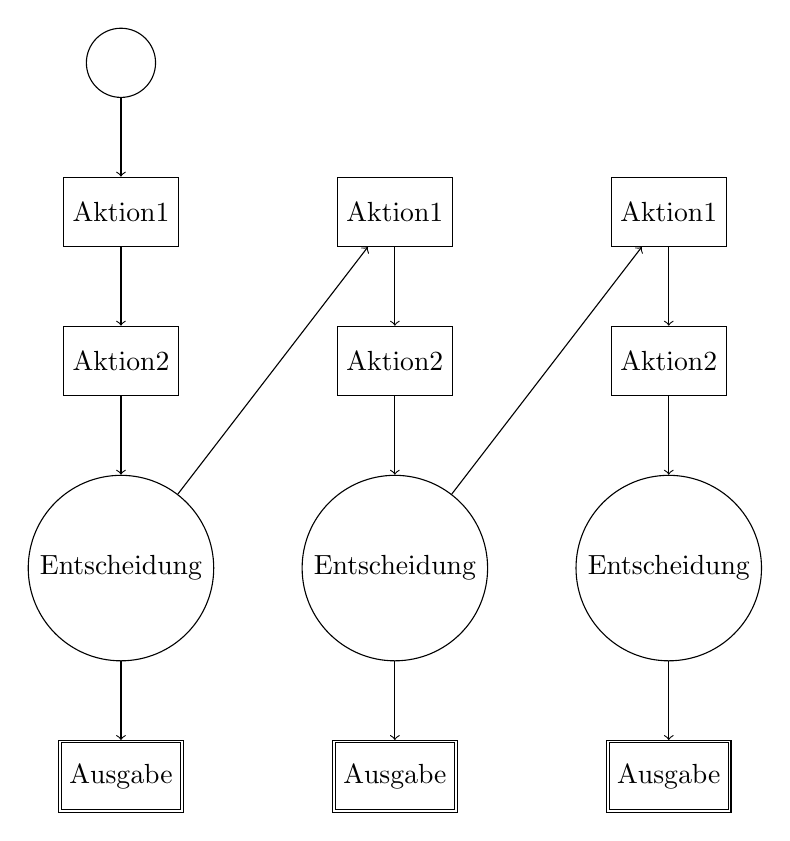
\begin{tikzpicture}[]
        \node[state, initial text=""](q5){};
        \node[state, rectangle, below = 1cm of q5](q6){Aktion1};
        \node[state, rectangle, below = 1cm of q6](q7){Aktion2};
        \node[state, below = 1cm of q7](q8){Entscheidung};
        \node[state, rectangle, accepting, below = 1cm of q8](q9){Ausgabe};

        \node[state, rectangle, right = 2cm of q6](q10){Aktion1};
        \node[state, rectangle, right = 2cm of q7](q11){Aktion2};
        \node[state, below = 1cm of q11](q12){Entscheidung};
        \node[state, rectangle, accepting, below = 1cm of q12](q13){Ausgabe};

        \node[state, rectangle, right = 2cm of q10](q14){Aktion1};
        \node[state, rectangle, right = 2cm of q11](q15){Aktion2};
        \node[state, below = 1cm of q15](q16){Entscheidung};
        \node[state, rectangle, accepting, below = 1cm of q16](q17){Ausgabe};

        \draw(q5) edge[->] (q6);
        \draw(q6) edge[->] (q7);
        \draw(q7) edge[->] (q8);
        \draw(q8) edge[->] (q9);
        \draw(q8) edge[->] (q10);
        
        \draw(q10) edge[->] (q11);
        \draw(q11) edge[->] (q12);
        \draw(q12) edge[->] (q13);
        \draw(q12) edge[->] (q14);

        \draw(q14) edge[->] (q15);
        \draw(q15) edge[->] (q16);
        \draw(q16) edge[->] (q17);


    \end{tikzpicture}
    }\\
    \textbf{Abbildung TODO}\\
    \subsection{2. Lösungsansatz}
    Schleife soll durch ein Konstrukt realisiert werden.
    Prüfungslogik muss um eine weitere Aktivitätsaktion erweitert werden. Das Schleifenkonstrukt greift dabei auf bereits vorhandene Regeln der Prüfungslogik zu.
    Das Schleifenkonstrukt greift dabei wie die anderen Aktivitätsaktionen auf den Referenzstack zu. Da der nächste Schleifendurchlauf nicht wieder auf den gleichen Eingabenwerten laufen soll, da diese wieder zu einem fehlerhaften Wert führen wird, muss ein Mechanismus im Schleifenkonstrukt implementiert werden, welcher einen neuen Wert holt.
    Durch die einführung der Schleife entstehen neue Herausforderungen. Es können nun Endlosschleifen entstehen, welche dazuführen dass die ausgeführte Prüfung niemals terminieren wird. Außerdem liefert der Hauptuntersuchungs-Adapter keine linearen Werte (?), sondern nicht determenistische Werte.

    Eine Endlosschleife kann von vorneherein ausgeschlossen werden, indem die maximalen Schleifendurchläufe begrenzt werden. 
    Da die Werte des Hauptuntersuchungs-Adapter nicht vorhersehbar sind und die Prüfung nicht jedes mal die maximale Anzahl der Schleifendurchläufe ausführen soll, muss ein Algorithmus entwickelt werden, welcher sagt wann man davon ausgehen kann, wann die ausgelesenen Sensorwerte sicht großartig nicht mehr ändern und stabil sind.
    
    Ein möglicher Lösungsvorschlag könnte nun folgendermaßen aussehen. 
    Je nachdem welcher Typ der Eingabewert hat verläuft der Algorithmus anders. Es wird dabei nur zwischen Zahlen und Zeichenketten unterschieden. 
    Bei Zeichenketten wird der aktuelle Wert mit dem Wert aus dem vorherigen Schleifendurchlauf verglichen. Dafür wird die Levenshtein-Distanz verwendet. Für die ersten beiden Schelifendurchläufe wird der Algorithmus übersprungen, weil die Levenshtein-Distanz noch kein Aussagekräftiges Ergebnis für den Anwendungsfall geben kann.
    Die Levenshtein-Distanz gibt die ähnlichkeit zwischen zwei Zeichenketten als Zahl an, indem sie die minimale Anzahl an Operation angibt, welche benötigt werden, damit die erste Zeichenkette der zweiten Zeichenkette gleicht. Je größer die Zahl ist destso "unterschiedlicher" sind die beiden Zeichenketten von einander. 

    Um zu schauen wie sich die Eingabe zu verschiedenen Zeiträumen verhält, berechnen wir Mittelwerte über TODO. Es sollten mindestens zwei Mittelwerte gebildet werden. Mehr als zwei Mittelwerte sind möglich, aber würden den Algorithmus entwindlicher machen. Der erste Mittelwert sollte über alle bisherigen Eingaben gebildet werden, um zu sehen wie sich die Eingabe auf langer Sicht verhält. Der zweite Mittelwert sollte über die letzten n Eingaben gebildert, um zu sehen wie sich die Eingabe auf kurzer Sicht verhält.
    Da die Werte der Levenshtein-Distanz sich für den Mittelwert nicht besonders anbieten, müssen die Zeichenketten in einen Zahlenwert umgewandelt werden.hließend Addieren. Für die Umwandlung eignet sich UTF-8 besonders gut. Da UTF-8 fast akke Schriftzeichen weltweit beinhaltet.
    Das kann geschaffen werden indem alle Zeichen der Zeichenkette in eine eindeutige Zahl umwandeln und die einzelnen Zahlen ansc
    Zusätzlich muss eine Gewichtung bei der Addition berücksichtigt werden, weil sonst Zeichenketten, die aus den gleichen Zeichen bestehen, den gleichen Wert bei der Addition rausbekommen. Das liegt daran, dass bei der Addition ohne Gewichtung nur die Wertigkeit der einzelnen Zeichen betrachtet wird, aber nicht deren Position. Dieses Problem wird mit der Gewichtung aufgelöst. Ein Beispiel dafür für die Addition mit Gewichtung ist in Abbildung TODO.
    Dies muss aber nicht für jedes Eingabepaar gemacht werden, sondern nur für Eingabepaare welche sich sehr ähneln, also eine niedrige Levenshtein-Distanz haben. Für Eingabepaare mit einer hohen Levenshtein-Distanz ist das nicht notwendig, weil wir da bereits wissen, dass sich die Zeichketten stark von einerander unterscheiden.
    Ist die Differenz aus der umgewandelten umgewandelten Zeichenkette und einem Mittel kleiner als ein vordefinierter Schwellenwert, wissen wir dass die Zeichenkette sich nur ganz leicht von den durchschnittlichen Eingaben unterscheidet.
    Wenn dies nun mehrmals nacheinander vorkommt, kann davon ausgegangen werden, dass der Wert in diesen Wertebereich stagniert.
    Um dies im ALgortithmus auch zu berücksichtigen, wird ein n-Chance Mechanismus eingebaut der folgendermaßen Funktioniert:
    \begin{itemize}
        \item Wird der Schwellenwert unterschritten, wird unser n dekrementiert.
        \item Wird der Schwellwert übertroffen oder ist unsere Differenz gleich wird n zurückgesetzt.
        \item Erreicht n irgendwann die 0 wird die Schleife abgebrochen. 
    \end{itemize}
    %Beispiel
    $
        "foo" = 102 + 111 + 111 = 324
        "oof" = 111 + 111 + 102 = 324
        mit Gewichtung
        "foo" = 1 * 102 + 2 * 111 + 3 * 111 = 657
        "oof" = 1 * 111 + 2 * 111 + 3 * 102 = 639
    $
    \\\textbf{Abbildung TODO} Beispiel Addition mit und ohne Gewichtung
    \\\\Ist unser Eingabewert nun keine Zeichenkette, sondern eine Zahl entfällt der Umwandlungsschritt mit der Gewichtung. Es kann sofort mit den beschriebenen Mittelwertansatz angefangen werden.
    %Schleifenkonstrukt -> Benutzer gibt Abbruchbedigung ein (Benutzer verwendet Schleifenkonstrukt statt Entscheidungs Aktivität) -> 
    %typ (generisch?, damit das System dies für uns übernimmt) der eingabe muss bestimmt werden, damit richtiger algorithmus zur stabilität überprüfung ausgewählt werden kann (es wird nur zwischen zeichenketten und zahlen unterschieden => bei zahlen wird mittelwertansatz gewählt bei zeichenketten Levenshtein-Distanz)
    %Was muss geändert werden: Prüfungslogik muss durch die aktivität schleife erweitert werden
    %Schluss
    \newpage
    \section{Evaluation}
    \label{Evaluation}
    \subsection{1. Lösungsansatz}
    +einfach zu implementieren, da wir kein schleifenkonstrukt mehr benötigen.
    +keine Endlosschleife, weil es keine Schleifen gibt
    +keine Zyklen, weil der Ablauf linear ist
    +weniger Sprünge, weil keine for oder while Bedingungen vorhanden sind
    +möglicher Performance gewinn, weil Schleifen-Overhead entfällt
    -größerer Codeumfang, da der eigentliche schleifenkörper a-mal im code implemtniert werden muss 
    -höherer verbraucht an ressourcen zB Speicher mehr code = mehr speicher
    -möglicherweise ineffizient, wenn der faktor zu groß gewählt wird
    -schlechtere Lesbarkeit
    -wenn bereits nach 3 durchlaufen feststeht, dass das gewünschte ergbeniss nicht mehr erreicht werden kann werden trotzdem die restlichen schritte ausgeführt
    \subsection{2. Lösungsansatz}
    +keine Endlosschleife, weil maximale Schleifendurchläufe begrenzt sind.
    +
    -azyklisches verhalten wird verletzt, weil schleifenkonstrukt benötigt wird
    -
    \newpage
    \renewcommand{\refname}{}
    \section{Literaturverzeichnis}
    \begin{thebibliography}{9}
        \bibitem{2}Johnston, W., Hanna, J., \& Millar, R. (2004). \emph{Advances in dataflow programming languages}. ACM Computing Surveys, 36(1), 1–34.
        \bibitem{3}Chen, L. (2021). \emph{Iteration vs. Recursion: Two Basic Algorithm Design Methodologies}. SIGACT News, 52(1), 81–86.
        \bibitem{4}Arvind, \& Culler, D. (1986). \emph{Dataflow Architectures}. LCS Technical Memos.
        \bibitem{5}Ambler, A., \& Burnett, M. (1990). \emph{Visual forms of iteration that preserve single assignment}. Journal of Visual Languages \& Computing, 1(2), 159–181.
        \bibitem{6}Mosconi, M., \& Porta, M. (2000). \emph{Iteration constructs in data-flow visual programming languages}. Computer Languages, 26(2), 67–104.
        \bibitem{1}Fan, Z., Li, W., Liu, T., Tang, S., Wang, Z., An, X., Ye, X., \& Fan, D. (2022). \emph{A Loop Optimization Method for Dataflow Architecture}. In 2022 IEEE 24th Int Conf on High Performance Computing \& Communications; 8th Int Conf on Data Science \& Systems; 20th Int Conf on Smart City; 8th Int Conf on Dependability in Sensor, Cloud \& Big Data Systems \& Application (HPCC/DSS/SmartCity/DependSys) (pp. 202–211).
        \bibitem{7}Gévay, G., Soto, J., \& Markl, V. (2021). \emph{Handling Iterations in Distributed Dataflow Systems}. ACM Comput. Surv., 54(9), 199:1–199:38.
        \bibitem{8}Alves, T., Marzulo, L., Kundu, S., \& França, F. (2021). \emph{Concurrency Analysis in Dynamic Dataflow Graphs}. IEEE Transactions on Emerging Topics in Computing, 9(1), 44–54.
        \bibitem{9}Ye, Z., \& Jiao, J. (2024). \emph{Loop Unrolling Based on SLP and Register Pressure Awareness}. In 2024 20th International Conference on Natural Computation, Fuzzy Systems and Knowledge Discovery (ICNC-FSKD) (pp. 1–6).
        \bibitem{10}Lučanin, D., \& Fabek, I. (2011). \emph{A visual programming language for drawing and executing flowcharts}. In 2011 Proceedings of the 34th International Convention MIPRO (pp. 1679–1684).
        \bibitem{11}Davis, A., \& Keller, R. (1982). \emph{Data Flow Program Graphs}. All HMC Faculty Publications and Research.
        \bibitem{21}Boshernitsan, M., \& Downes, M. (2004). \emph{Visual Programming Languages: A Survey}. EECS University of California, Berkeley.
        \bibitem{12}Charntaweekhun, K., \& Wangsiripitak, S. (2006). \emph{Visual Programming using Flowchart}. In 2006 International Symposium on Communications and Information Technologies (pp. 1062–1065).
        \bibitem{13}Burnett, M., Baker, M., Bohus, C., Carlson, P., Yang, S., \& Van Zee, P. (1995). \emph{Scaling up visual programming languages}. Computer, 28(3), 45–54.
        \bibitem{14}Kurihara, A., Sasaki, A., Wakita, K., \& Hosobe, H. (2015). \emph{A Programming Environment for Visual Block-Based Domain-Specific Languages}. Procedia Computer Science, 62, 287–296.
        \bibitem{15}Hils, D. (1992). \emph{Visual languages and computing survey: Data flow visual programming languages}. Journal of Visual Languages \& Computing, 3(1), 69–101.
        \bibitem{19}Sousa, T. (2012). \emph{Dataflow Programming Concept, Languages and Applications}. Doctoral Symposium on Informatics Engineering, 7.
        \bibitem{18}Van Deursen, A., Klint, P., \& Visser, J. (2000). \emph{Domain-specific languages: an annotated bibliography}. ACM SIGPLAN Notices, 35(6), 26–36.
        \bibitem{16}Roy, G., Kelso, J., \& Standing, C. (1998). \emph{Towards a visual programming environment for software development}. In Proceedings. 1998 International Conference Software Engineering: Education and Practice (Cat. No.98EX220) (pp. 381–388). IEEE Comput. Soc.
        \bibitem{20}Weintrop, D. (2019). \emph{Block-based programming in computer science education}. Communications of the ACM, 62(8), 22–25.
        \bibitem{22}Gumm, H.P., \& Sommer, M. (2016). \emph{Band 1 Programmierung, Algorithmen und Datenstrukturen}. De Gruyter Oldenbourg.
    \end{thebibliography}
\end{document}    